\section{Installationsanleitung für MySQL}

\subsection{Installation}

\subsubsection{Installation von MySQL}

Im Kursverzeichnis findest du im Ordner \myFile{32\_SQL\_Einfuehrung} und dort
im Ordner \myFile{Installationsdateien}\footnote{oder alternativ auch hier:
\url{http://dev.mysql.com/downloads/installer/}} die Datei
\myFile{mysql-installer-web-community-5.6.26.0.msi}. Dabei handelt es sich um
ein kleines Windows-Programm welches den Download und die Installation der
eigentlichen MySQL Programme bequem erledigt.

Im Prinzip kannst du dich einfach durchklicken. Nur dann, wenn nach dem Passwort
für den root Benutzer für MySQL gefragt wird, musst du etwas eingeben: 

Bei \myPMI{Current Root Passwort} gibst du entweder nichts ein (wenn dies die
erste Installation von MySQL auf deinem Rechner ist) oder das alte
Root-Passwort. Bei \myPMI{MySQL Root Password} und \myPMI{Repeat Password} gibst
du jeweils \myUserInput{root} ein.


\subsubsection{Installation des Java-Treibers}

Um von einem Java-Programm aus auf MySQL zugreifen zu können, muss man einen speziellen Treiber
installieren, und in Eclipse einbinden (siehe einleitendes Kapitel zur
Konfiguration von Eclipse).

Im selben Ordner wie zuvor den MySQL-Installer findest auch den MySQL
JDBC-Connectors:

\myFile{mysql-connector-java-5.1.36-bin.jar}

Dieses Java Archiv muss in euer eigenes Java-Projekt in Eclipse eingebunden
werden, damit ihr später aus eueren Java-Programmen heraus auf den MySQL-Server
zugreifen könnt. Siehe Kapitel \ref{mysql-connector-installation}.


% \subsection{Benutzung von MySQL-Workbench}
% 
% \subsubsection{Anmelden}
% 
% \begin{tabular}{ll}
% Host:           & \myUserInput{localhost}\\
% Port:           & \myUserInput{3306}\\
% Nutzername:     & \myUserInput{root}\\
% Passwort:       & \myUserInput{root}\\
% Standardschema: & Die gewünschte Datenbank -- Feld kann leer bleiben\\
% \end{tabular}
% 
% Ein Klick auf das blau hinterlegte \myPMI{Local Instance MySQL} im linken Teil
% des Fensters reicht!
% 
% 
% \subsubsection{„Safe Update Mode“ deaktivieren}
% 
% Wenn du MySQL-Workbench zum ersten mal startest, solltest du \textbf{unbedingt
% den sogenannten „Safe Update Mode“ deaktivieren} (ansonsten werden die meisten
% SQL-Befehle nicht funktionieren). Das tust du wie folgt:
% 
% \myPMI{Edit} $\rightarrow$ \myPMI{Preferences} $\rightarrow$ \myPMI{SQL Queries}
% 
% und dort das Häkchen vor \myPMI{$<$“Safe Updates“. Forbid UPDATE and DELETE
% statements without \ldots$>$} entfernen.
% 
% \begin{center}
% 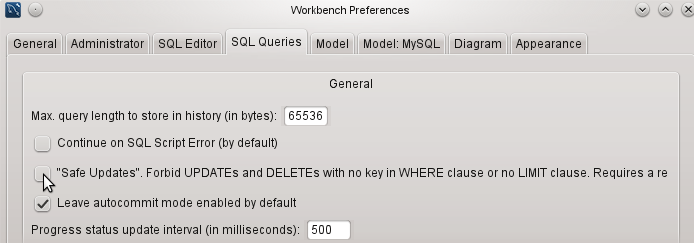
\includegraphics[width=0.9\textwidth]{./inf/SEKII/32_SQL_Einfuehrung/workbench_safe_updates.png}
% \end{center}
% 
% Anschließend musst du MySQL-Workbench einmal neu starten.
% 
% 
% \subsubsection{Bedienung}
% 
% Im mittleren Feld (Reiter \myPMI{Query 1}) kann man nun direkt SQL-Kommandos
% eingeben. Die Befehle können durch einen Klick auf den „Blitz“ ausgeführt
% werden.
% 
% \subsubsection{SQL-Anweisungen aus einer Datei einfügen} 
% 
% SQL-Befehle können auch in einer Datei als Skript gespeichert werden bzw. aus
% einem SQL-Skript (Dateiendung \myFile{*.sql}) geladen werden. Wenn einzelne
% Zeilen in der Datei beim Test nicht ausgeführt werden sollen, fügt man an den
% Anfang der Zeile das Zeichen \myUserInput{\#} ein, um aus dem Code einen
% Kommentar zu machen.
% 
% Gehe folgendermaßen vor, um den Code aus der Datei auszuführen:
% 
% \begin{compactenum}
%   
% \item Menüpunkt \myPMI{File} $\rightarrow$ \myPMI{Open SQL Script \ldots} wählen
% und die Datei laden (die Datei hat üblicherweise die Endung \myFile{*.sql}).
% 
% \item In der Toolbar auf \myPMI{Ausführen} klicken (Blitz-Symbol).
% 
% \end{compactenum}